\begin{frame}[fragile]{The asphalt data}
\protect\hypertarget{the-asphalt-data}{}
\begin{itemize}
\tightlist
\item
  31 asphalt pavements prepared under different conditions. How does
  quality of pavement depend on these?
\item
  Variables:

  \begin{itemize}
  \tightlist
  \item
    \texttt{pct.a.surf} The percentage of asphalt in the surface layer
  \item
    \texttt{pct.a.base} The percentage of asphalt in the base layer
  \item
    \texttt{fines} The percentage of fines in the surface layer
  \item
    \texttt{voids} The percentage of voids in the surface layer
  \item
    \texttt{rut.depth} The change in rut depth per million vehicle
    passes
  \item
    \texttt{viscosity} The viscosity of the asphalt
  \item
    \texttt{run} 2 data collection periods: run 1 for run 1, 0 for run
    2.
  \end{itemize}
\item
  \texttt{rut.depth} response. Depends on other variables, how?
\end{itemize}
\end{frame}

\begin{frame}[fragile]{Packages for this section}
\protect\hypertarget{packages-for-this-section}{}
\begin{Shaded}
\begin{Highlighting}[]
\KeywordTok{library}\NormalTok{(MASS)}
\KeywordTok{library}\NormalTok{(tidyverse)}
\KeywordTok{library}\NormalTok{(broom)}
\KeywordTok{library}\NormalTok{(leaps)}
\end{Highlighting}
\end{Shaded}
\end{frame}

\begin{frame}[fragile]{Getting set up}
\protect\hypertarget{getting-set-up}{}
\begin{Shaded}
\begin{Highlighting}[]
\NormalTok{my\_url \textless{}{-}}\StringTok{ "http://www.utsc.utoronto.ca/\textasciitilde{}butler/c32/asphalt.txt"}
\NormalTok{asphalt \textless{}{-}}\StringTok{ }\KeywordTok{read\_delim}\NormalTok{(my\_url, }\StringTok{" "}\NormalTok{)}
\end{Highlighting}
\end{Shaded}

\begin{verbatim}
## Parsed with column specification:
## cols(
##   pct.a.surf = col_double(),
##   pct.a.base = col_double(),
##   fines = col_double(),
##   voids = col_double(),
##   rut.depth = col_double(),
##   viscosity = col_double(),
##   run = col_double()
## )
\end{verbatim}

\begin{itemize}
\tightlist
\item
  Quantitative variables with one response: multiple regression.
\item
  Some issues here that don't come up in ``simple'' regression; handle
  as we go. (STAB27/STAC67 ideas.)
\end{itemize}
\end{frame}

\begin{frame}[fragile]{The data (some)}
\protect\hypertarget{the-data-some}{}
\begin{Shaded}
\begin{Highlighting}[]
\NormalTok{asphalt}
\end{Highlighting}
\end{Shaded}

\begin{longtable}[]{@{}rrrrrrr@{}}
\toprule
pct.a.surf & pct.a.base & fines & voids & rut.depth & viscosity &
run\tabularnewline
\midrule
\endhead
4.68 & 4.87 & 8.4 & 4.916 & 6.75 & 2.80 & 1\tabularnewline
5.19 & 4.50 & 6.5 & 4.563 & 13.00 & 1.40 & 1\tabularnewline
4.82 & 4.73 & 7.9 & 5.321 & 14.75 & 1.40 & 1\tabularnewline
4.85 & 4.76 & 8.3 & 4.865 & 12.60 & 3.30 & 1\tabularnewline
4.86 & 4.95 & 8.4 & 3.776 & 8.25 & 1.70 & 1\tabularnewline
5.16 & 4.45 & 7.4 & 4.397 & 10.67 & 2.90 & 1\tabularnewline
4.82 & 5.05 & 6.8 & 4.867 & 7.28 & 3.70 & 1\tabularnewline
4.86 & 4.70 & 8.6 & 4.828 & 12.67 & 1.70 & 1\tabularnewline
4.78 & 4.84 & 6.7 & 4.865 & 12.58 & 0.92 & 1\tabularnewline
5.16 & 4.76 & 7.7 & 4.034 & 20.60 & 0.68 & 1\tabularnewline
4.57 & 4.82 & 7.4 & 5.450 & 3.58 & 6.00 & 1\tabularnewline
4.61 & 4.65 & 6.7 & 4.853 & 7.00 & 4.30 & 1\tabularnewline
5.07 & 5.10 & 7.5 & 4.257 & 26.20 & 0.60 & 1\tabularnewline
4.66 & 5.09 & 8.2 & 5.144 & 11.67 & 1.80 & 1\tabularnewline
5.42 & 4.41 & 5.8 & 3.718 & 7.67 & 6.00 & 1\tabularnewline
5.01 & 4.74 & 7.1 & 4.715 & 12.25 & 4.40 & 1\tabularnewline
4.97 & 4.66 & 6.5 & 4.625 & 0.76 & 88.00 & 0\tabularnewline
4.01 & 4.72 & 8.0 & 4.977 & 1.35 & 62.00 & 0\tabularnewline
4.96 & 4.90 & 6.8 & 4.322 & 1.44 & 50.00 & 0\tabularnewline
5.20 & 4.70 & 8.2 & 5.087 & 1.60 & 58.00 & 0\tabularnewline
4.80 & 4.60 & 6.6 & 5.971 & 1.10 & 90.00 & 0\tabularnewline
4.98 & 4.69 & 6.4 & 4.647 & 0.85 & 66.00 & 0\tabularnewline
5.35 & 4.76 & 7.3 & 5.115 & 1.20 & 140.00 & 0\tabularnewline
5.04 & 4.80 & 7.8 & 5.939 & 0.56 & 240.00 & 0\tabularnewline
4.80 & 4.80 & 7.4 & 5.916 & 0.72 & 420.00 & 0\tabularnewline
4.83 & 4.60 & 6.7 & 5.471 & 0.47 & 500.00 & 0\tabularnewline
4.66 & 4.72 & 7.2 & 4.602 & 0.33 & 180.00 & 0\tabularnewline
4.67 & 4.50 & 6.3 & 5.043 & 0.26 & 270.00 & 0\tabularnewline
4.72 & 4.70 & 6.8 & 5.075 & 0.76 & 170.00 & 0\tabularnewline
5.00 & 5.07 & 7.2 & 4.334 & 0.80 & 98.00 & 0\tabularnewline
4.70 & 4.80 & 7.7 & 5.705 & 2.00 & 35.00 & 0\tabularnewline
\bottomrule
\end{longtable}
\end{frame}

\begin{frame}[fragile]{Plotting response ``rut depth'' against
everything else}
\protect\hypertarget{plotting-response-rut-depth-against-everything-else}{}
Same idea as for plotting separate predictions on one plot:

\begin{Shaded}
\begin{Highlighting}[]
\NormalTok{asphalt }\OperatorTok{\%\textgreater{}\%}
\StringTok{  }\KeywordTok{pivot\_longer}\NormalTok{(}
    \OperatorTok{{-}}\NormalTok{rut.depth,}
    \DataTypeTok{names\_to=}\StringTok{"xname"}\NormalTok{, }\DataTypeTok{values\_to=}\StringTok{"x"}
\NormalTok{  ) }\OperatorTok{\%\textgreater{}\%}
\StringTok{  }\KeywordTok{ggplot}\NormalTok{(}\KeywordTok{aes}\NormalTok{(}\DataTypeTok{x =}\NormalTok{ x, }\DataTypeTok{y =}\NormalTok{ rut.depth)) }\OperatorTok{+}\StringTok{ }\KeywordTok{geom\_point}\NormalTok{() }\OperatorTok{+}
\StringTok{  }\KeywordTok{facet\_wrap}\NormalTok{(}\OperatorTok{\textasciitilde{}}\NormalTok{xname, }\DataTypeTok{scales =} \StringTok{"free"}\NormalTok{) {-}\textgreater{}}\StringTok{ }\NormalTok{g}
\end{Highlighting}
\end{Shaded}

``collect all the x-variables together into one column called x, with
another column xname saying which x they were, then plot these x's
against rut.depth, a separate facet for each x-variable.''

I saved this graph to plot later (on the next page).
\end{frame}

\begin{frame}[fragile]{The plot}
\protect\hypertarget{the-plot}{}
\begin{Shaded}
\begin{Highlighting}[]
\NormalTok{g}
\end{Highlighting}
\end{Shaded}

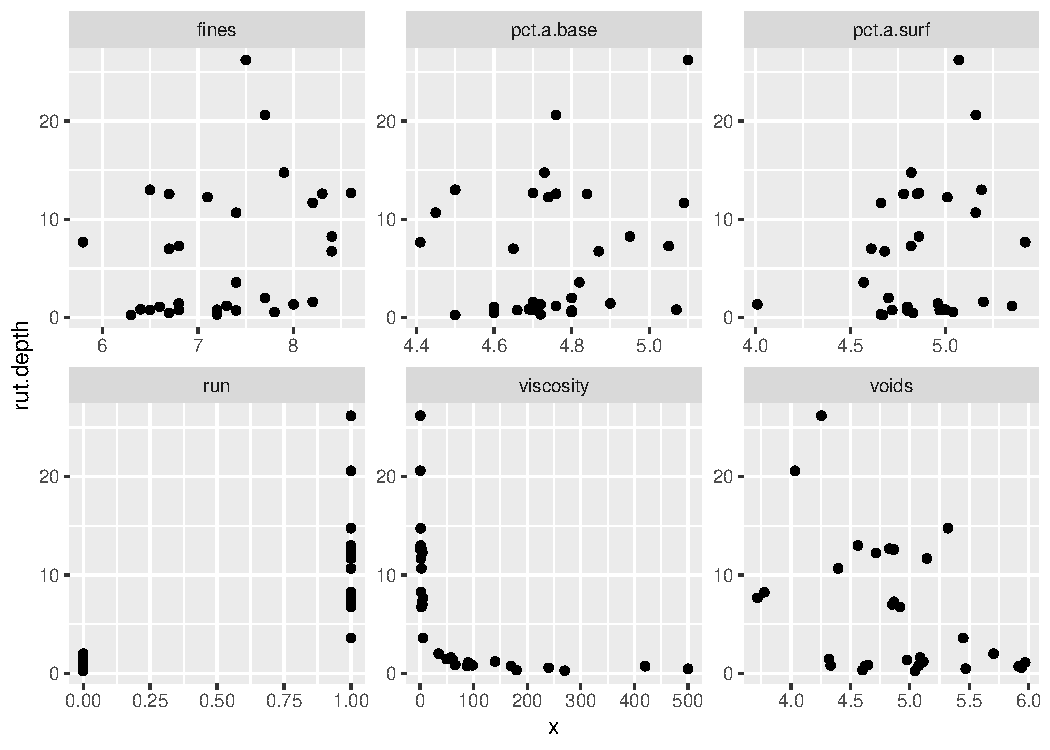
\includegraphics{asphalt_slides_files/figure-beamer/unnamed-chunk-8-1.pdf}
\end{frame}

\begin{frame}[fragile]{Interpreting the plots}
\protect\hypertarget{interpreting-the-plots}{}
\begin{itemize}
\tightlist
\item
  One plot of rut depth against each of the six other variables.
\item
  Get rough idea of what's going on.
\item
  Trends mostly weak.
\item
  \texttt{viscosity} has strong but non-linear trend.
\item
  \texttt{run} has effect but variability bigger when run is 1.
\item
  Weak but downward trend for \texttt{voids}.
\item
  Non-linearity of \texttt{rut.depth}-\texttt{viscosity} relationship
  should concern us.
\item
  Take this back to asphalt engineer: suggests log of
  \texttt{viscosity}:
\end{itemize}

\begin{Shaded}
\begin{Highlighting}[]
\KeywordTok{ggplot}\NormalTok{(asphalt, }\KeywordTok{aes}\NormalTok{(}\DataTypeTok{y =}\NormalTok{ rut.depth, }\DataTypeTok{x =} \KeywordTok{log}\NormalTok{(viscosity))) }\OperatorTok{+}
\StringTok{  }\KeywordTok{geom\_point}\NormalTok{() }\OperatorTok{+}\StringTok{ }\KeywordTok{geom\_smooth}\NormalTok{(}\DataTypeTok{se =}\NormalTok{ F)}
\end{Highlighting}
\end{Shaded}

(plot overleaf)
\end{frame}

\begin{frame}{Rut depth against log-viscosity}
\protect\hypertarget{rut-depth-against-log-viscosity}{}
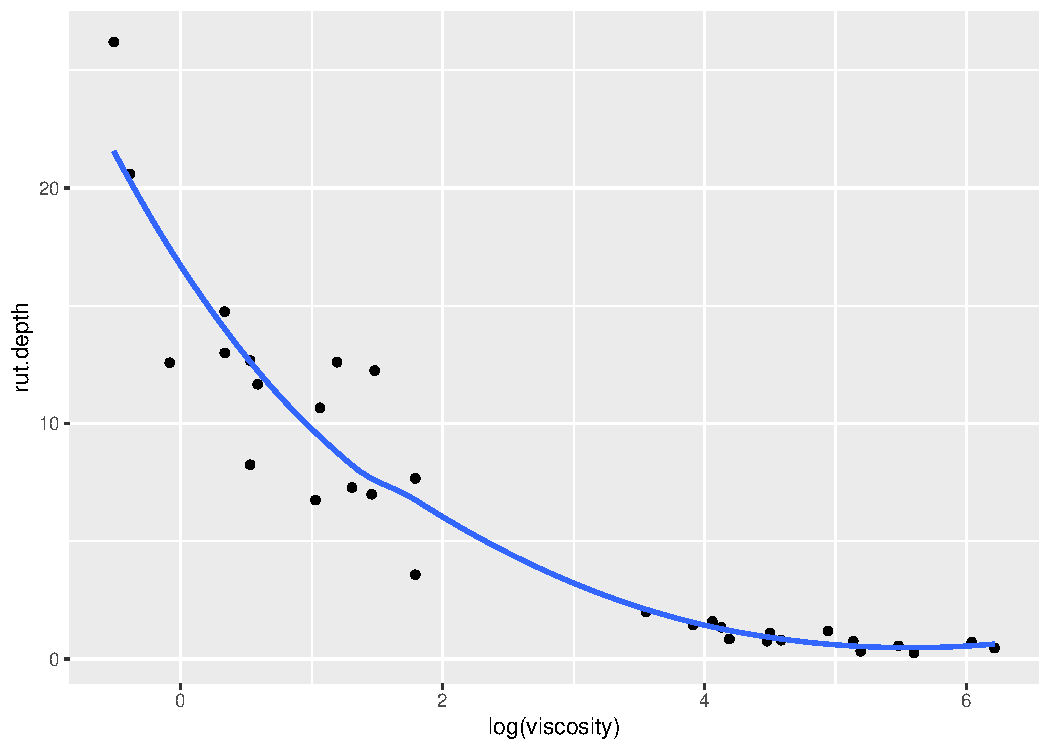
\includegraphics{asphalt_slides_files/figure-beamer/unnamed-chunk-9-1.pdf}
\end{frame}

\begin{frame}[fragile]{Comments and next steps}
\protect\hypertarget{comments-and-next-steps}{}
\begin{itemize}
\tightlist
\item
  Not very linear, but better than before.
\item
  In multiple regression, hard to guess which x's affect response. So
  typically start by predicting from everything else.
\item
  Model formula has response on left, squiggle, explanatories on right
  joined by plusses:
\end{itemize}

\begin{Shaded}
\begin{Highlighting}[]
\NormalTok{rut}\FloatTok{.1}\NormalTok{ \textless{}{-}}\StringTok{ }\KeywordTok{lm}\NormalTok{(rut.depth }\OperatorTok{\textasciitilde{}}\StringTok{ }\NormalTok{pct.a.surf }\OperatorTok{+}\StringTok{ }\NormalTok{pct.a.base }\OperatorTok{+}\StringTok{ }\NormalTok{fines }\OperatorTok{+}
\StringTok{  }\NormalTok{voids }\OperatorTok{+}\StringTok{ }\KeywordTok{log}\NormalTok{(viscosity) }\OperatorTok{+}\StringTok{ }\NormalTok{run, }\DataTypeTok{data =}\NormalTok{ asphalt)}
\end{Highlighting}
\end{Shaded}
\end{frame}

\begin{frame}[fragile]{Regression output: \texttt{summary(rut.1)} or:}
\protect\hypertarget{regression-output-summaryrut.1-or}{}
\footnotesize

\begin{Shaded}
\begin{Highlighting}[]
\KeywordTok{glance}\NormalTok{(rut}\FloatTok{.1}\NormalTok{)}
\end{Highlighting}
\end{Shaded}

\begin{longtable}[]{@{}rrrrrrrrrrr@{}}
\toprule
r.squared & adj.r.squared & sigma & statistic & p.value & df & logLik &
AIC & BIC & deviance & df.residual\tabularnewline
\midrule
\endhead
0.8060035 & 0.7575043 & 3.323526 & 16.61893 & 2e-07 & 7 & -77.25194 &
170.5039 & 181.9758 & 265.0998 & 24\tabularnewline
\bottomrule
\end{longtable}

\begin{Shaded}
\begin{Highlighting}[]
\KeywordTok{tidy}\NormalTok{(rut}\FloatTok{.1}\NormalTok{)}
\end{Highlighting}
\end{Shaded}

\begin{longtable}[]{@{}lrrrr@{}}
\toprule
term & estimate & std.error & statistic & p.value\tabularnewline
\midrule
\endhead
(Intercept) & -12.9936763 & 26.2187822 & -0.4955866 &
0.6246937\tabularnewline
pct.a.surf & 3.9705671 & 2.4966454 & 1.5903608 &
0.1248412\tabularnewline
pct.a.base & 1.2631409 & 3.9702906 & 0.3181482 &
0.7531244\tabularnewline
fines & 0.1164434 & 1.0123885 & 0.1150185 & 0.9093873\tabularnewline
voids & 0.5892602 & 1.3243933 & 0.4449284 & 0.6603584\tabularnewline
log(viscosity) & -3.1515128 & 0.9194468 & -3.4276183 &
0.0022027\tabularnewline
run & -1.9654795 & 3.6472048 & -0.5389002 & 0.5949198\tabularnewline
\bottomrule
\end{longtable}

\normalsize
\end{frame}

\begin{frame}[fragile]{Comments}
\protect\hypertarget{comments}{}
\begin{itemize}
\tightlist
\item
  R-squared 81\%, not so bad.
\item
  P-value in \texttt{glance} asserts that something helping to predict
  rut.depth.
\item
  Table of coefficients says \texttt{log(viscosity)}.
\item
  But confused by clearly non-significant variables: remove those to get
  clearer picture of what is helpful.
\item
  Before we do anything, look at residual plots:

  \begin{itemize}
  \item
    \begin{enumerate}
    [(a)]
    \tightlist
    \item
      of residuals against fitted values (as usual)
    \end{enumerate}
  \item
    \begin{enumerate}
    [(a)]
    \setcounter{enumi}{1}
    \tightlist
    \item
      of residuals against each explanatory.
    \end{enumerate}
  \end{itemize}
\item
  Problem fixes:

  \begin{itemize}
  \tightlist
  \item
    with (a): fix response variable;
  \item
    with some plots in (b): fix those explanatory variables.
  \end{itemize}
\end{itemize}
\end{frame}

\begin{frame}[fragile]{Plot fitted values against residuals}
\protect\hypertarget{plot-fitted-values-against-residuals}{}
\begin{Shaded}
\begin{Highlighting}[]
\KeywordTok{ggplot}\NormalTok{(rut}\FloatTok{.1}\NormalTok{, }\KeywordTok{aes}\NormalTok{(}\DataTypeTok{x =}\NormalTok{ .fitted, }\DataTypeTok{y =}\NormalTok{ .resid)) }\OperatorTok{+}\StringTok{ }\KeywordTok{geom\_point}\NormalTok{()}
\end{Highlighting}
\end{Shaded}

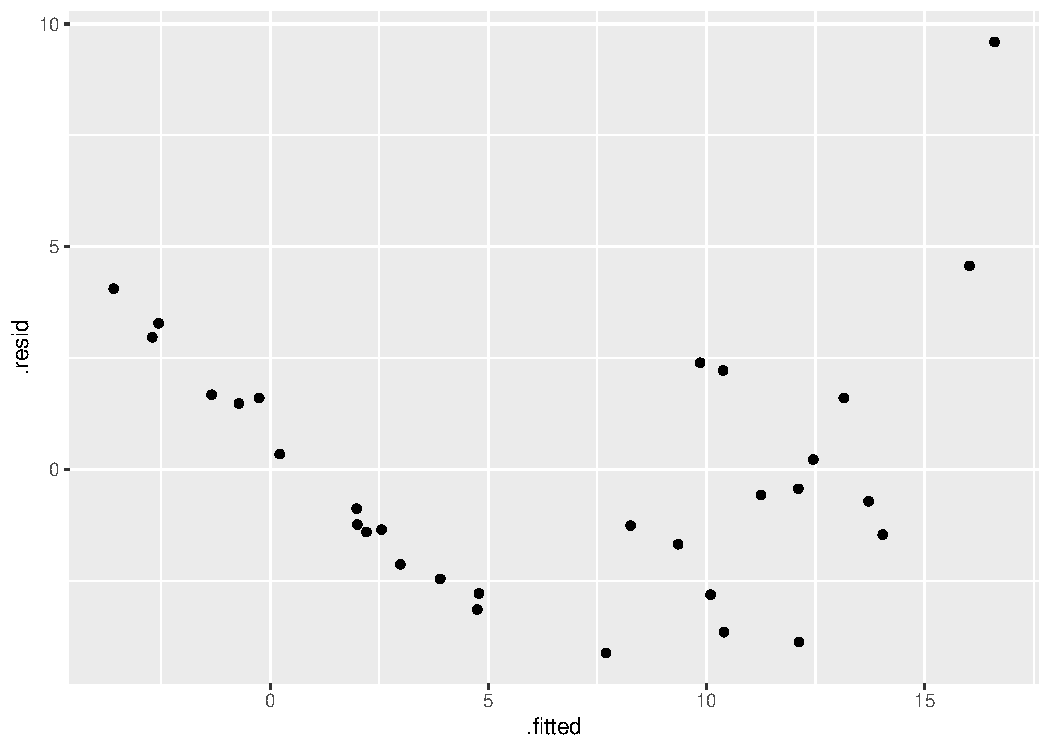
\includegraphics{asphalt_slides_files/figure-beamer/unnamed-chunk-12-1.pdf}
\end{frame}

\begin{frame}[fragile]{Plotting residuals against \(x\) variables}
\protect\hypertarget{plotting-residuals-against-x-variables}{}
\begin{itemize}
\tightlist
\item
  Problem here is that residuals are in the fitted model, and the
  observed \(x\)-values are in the original data frame \texttt{asphalt}.
\item
  Package broom contains a function \texttt{augment} that combines these
  two together so that they can later be plotted: start with a model
  first, and then augment with a data frame:
\end{itemize}

\begin{Shaded}
\begin{Highlighting}[]
\NormalTok{rut}\FloatTok{.1} \OperatorTok{\%\textgreater{}\%}\StringTok{ }\KeywordTok{augment}\NormalTok{(asphalt) {-}\textgreater{}}\StringTok{ }\NormalTok{rut}\FloatTok{.1}\NormalTok{a}
\end{Highlighting}
\end{Shaded}
\end{frame}

\begin{frame}[fragile]{What does rut.1a contain?}
\protect\hypertarget{what-does-rut.1a-contain}{}
\begin{Shaded}
\begin{Highlighting}[]
\KeywordTok{names}\NormalTok{(rut}\FloatTok{.1}\NormalTok{a)}
\end{Highlighting}
\end{Shaded}

\begin{verbatim}
##  [1] "pct.a.surf" "pct.a.base" "fines"     
##  [4] "voids"      "rut.depth"  "viscosity" 
##  [7] "run"        ".fitted"    ".se.fit"   
## [10] ".resid"     ".hat"       ".sigma"    
## [13] ".cooksd"    ".std.resid"
\end{verbatim}

\begin{itemize}
\tightlist
\item
  all the stuff in original data frame, plus:
\item
  quantities from regression (starting with a dot)
\end{itemize}
\end{frame}

\begin{frame}[fragile]{Plotting residuals against \(x\)-variables}
\protect\hypertarget{plotting-residuals-against-x-variables-1}{}
\begin{Shaded}
\begin{Highlighting}[]
\NormalTok{rut}\FloatTok{.1}\NormalTok{a }\OperatorTok{\%\textgreater{}\%}
\StringTok{  }\KeywordTok{mutate}\NormalTok{(}\DataTypeTok{log\_vis=}\KeywordTok{log}\NormalTok{(viscosity)) }\OperatorTok{\%\textgreater{}\%}\StringTok{ }
\StringTok{  }\KeywordTok{pivot\_longer}\NormalTok{(}
    \KeywordTok{c}\NormalTok{(pct.a.surf}\OperatorTok{:}\NormalTok{voids, run, log\_vis),}
    \DataTypeTok{names\_to=}\StringTok{"xname"}\NormalTok{, }\DataTypeTok{values\_to=}\StringTok{"x"}
\NormalTok{  ) }\OperatorTok{\%\textgreater{}\%}
\StringTok{  }\KeywordTok{ggplot}\NormalTok{(}\KeywordTok{aes}\NormalTok{(}\DataTypeTok{x =}\NormalTok{ x, }\DataTypeTok{y =}\NormalTok{ .resid)) }\OperatorTok{+}
\StringTok{  }\KeywordTok{geom\_point}\NormalTok{() }\OperatorTok{+}\StringTok{ }\KeywordTok{facet\_wrap}\NormalTok{(}\OperatorTok{\textasciitilde{}}\NormalTok{xname, }\DataTypeTok{scales =} \StringTok{"free"}\NormalTok{) {-}\textgreater{}}\StringTok{ }\NormalTok{g}
\end{Highlighting}
\end{Shaded}
\end{frame}

\begin{frame}[fragile]{The plot}
\protect\hypertarget{the-plot-1}{}
\begin{Shaded}
\begin{Highlighting}[]
\NormalTok{g}
\end{Highlighting}
\end{Shaded}

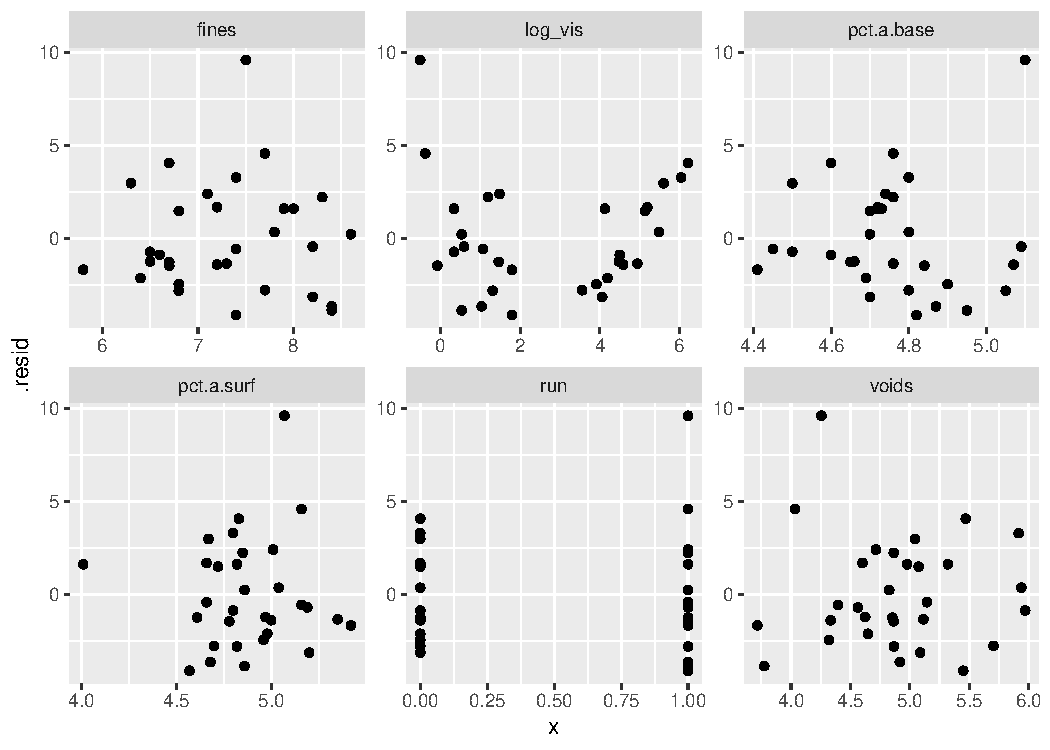
\includegraphics{asphalt_slides_files/figure-beamer/unnamed-chunk-17-1.pdf}
\end{frame}

\begin{frame}{Comments}
\protect\hypertarget{comments-1}{}
\begin{itemize}
\tightlist
\item
  There is serious curve in plot of residuals vs.~fitted values.
  Suggests a transformation of \(y\).
\item
  The residuals-vs-\(x\)'s plots don't show any serious trends. Worst
  probably that potential curve against log-viscosity.
\item
  Also, large positive residual, 10, that shows up on all plots. Perhaps
  transformation of \(y\) will help with this too.
\item
  If residual-fitted plot OK, but some residual-\(x\) plots not, try
  transforming those \(x\)'s, eg. by adding \(x^2\) to help with curve.
\end{itemize}
\end{frame}

\begin{frame}{Which transformation?}
\protect\hypertarget{which-transformation}{}
\begin{itemize}
\tightlist
\item
  Best way: consult with person who brought you the data.
\item
  Can't do that here!
\item
  No idea what transformation would be good.
\item
  Let data choose: ``Box-Cox transformation''.
\item
  Scale is that of ``ladder of powers'': power transformation, but 0 is
  log.
\end{itemize}
\end{frame}

\begin{frame}[fragile]{Running Box-Cox}
\protect\hypertarget{running-box-cox}{}
From package \texttt{MASS}:

\begin{Shaded}
\begin{Highlighting}[]
\KeywordTok{boxcox}\NormalTok{(rut.depth }\OperatorTok{\textasciitilde{}}\StringTok{ }\NormalTok{pct.a.surf }\OperatorTok{+}\StringTok{ }\NormalTok{pct.a.base }\OperatorTok{+}\StringTok{ }\NormalTok{fines }\OperatorTok{+}\StringTok{ }\NormalTok{voids }\OperatorTok{+}
\StringTok{  }\KeywordTok{log}\NormalTok{(viscosity) }\OperatorTok{+}\StringTok{ }\NormalTok{run, }\DataTypeTok{data =}\NormalTok{ asphalt)}
\end{Highlighting}
\end{Shaded}

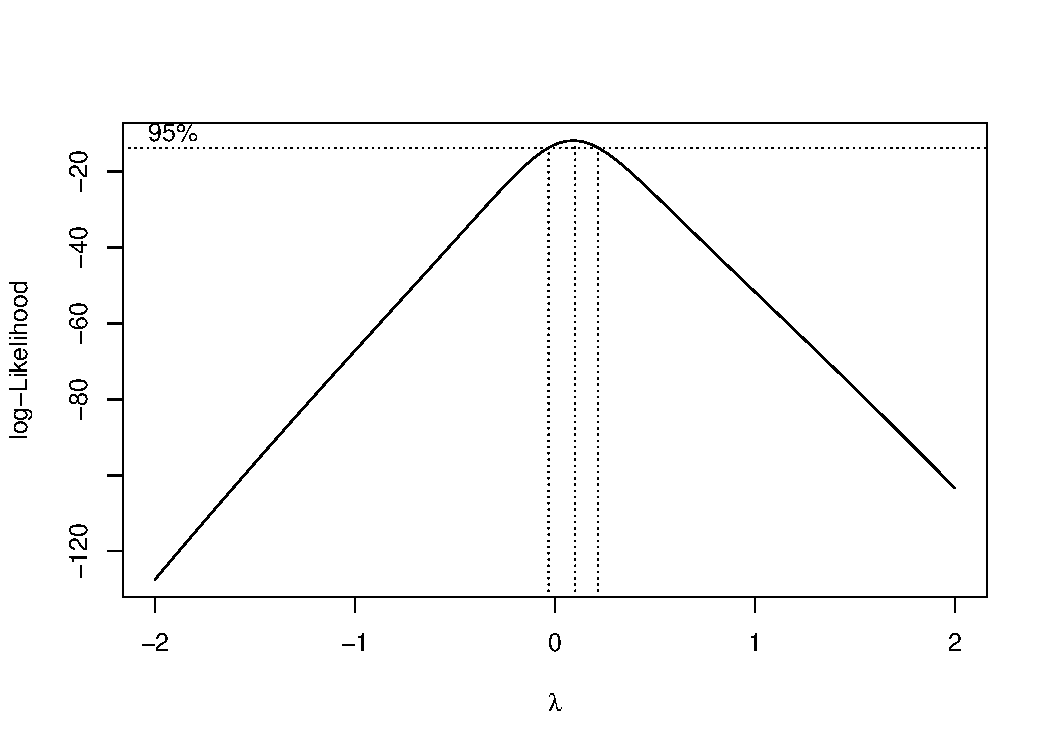
\includegraphics{asphalt_slides_files/figure-beamer/unnamed-chunk-18-1.pdf}
\end{frame}

\begin{frame}{Comments on Box-Cox plot}
\protect\hypertarget{comments-on-box-cox-plot}{}
\begin{itemize}
\tightlist
\item
  \(\lambda\) represents power to transform \(y\) with.
\item
  Best single choice of transformation parameter \(\lambda\) is peak of
  curve, close to 0.
\item
  Vertical dotted lines give CI for \(\lambda\), about (−0.05, 0.2).
\item
  \(\lambda = 0\) means ``log''.
\item
  Narrowness of confidence interval mean that these not supported by
  data:

  \begin{itemize}
  \tightlist
  \item
    No transformation (\(\lambda = 1\))
  \item
    Square root (\(\lambda = 0.5\))
  \item
    Reciprocal (\(\lambda = −1\)).
  \end{itemize}
\end{itemize}
\end{frame}

\begin{frame}[fragile]{Relationships with explanatories}
\protect\hypertarget{relationships-with-explanatories}{}
\begin{itemize}
\tightlist
\item
  As before: plot response (now \texttt{log(rut.depth)}) against other
  explanatory variables, all in one shot:
\end{itemize}

\begin{Shaded}
\begin{Highlighting}[]
\NormalTok{asphalt }\OperatorTok{\%\textgreater{}\%}
\StringTok{  }\KeywordTok{mutate}\NormalTok{(}\DataTypeTok{log\_vis=}\KeywordTok{log}\NormalTok{(viscosity)) }\OperatorTok{\%\textgreater{}\%}\StringTok{ }
\StringTok{  }\KeywordTok{pivot\_longer}\NormalTok{(}
    \KeywordTok{c}\NormalTok{(pct.a.surf}\OperatorTok{:}\NormalTok{voids, run, log\_vis),}
    \DataTypeTok{names\_to=}\StringTok{"xname"}\NormalTok{, }\DataTypeTok{values\_to=}\StringTok{"x"}
\NormalTok{  ) }\OperatorTok{\%\textgreater{}\%}
\StringTok{  }\KeywordTok{ggplot}\NormalTok{(}\KeywordTok{aes}\NormalTok{(}\DataTypeTok{y =} \KeywordTok{log}\NormalTok{(rut.depth), }\DataTypeTok{x =}\NormalTok{ x)) }\OperatorTok{+}\StringTok{ }\KeywordTok{geom\_point}\NormalTok{() }\OperatorTok{+}
\StringTok{  }\KeywordTok{facet\_wrap}\NormalTok{(}\OperatorTok{\textasciitilde{}}\NormalTok{xname, }\DataTypeTok{scales =} \StringTok{"free"}\NormalTok{) {-}\textgreater{}}\StringTok{ }\NormalTok{g3}
\end{Highlighting}
\end{Shaded}
\end{frame}

\begin{frame}[fragile]{The new plots}
\protect\hypertarget{the-new-plots}{}
\begin{Shaded}
\begin{Highlighting}[]
\NormalTok{g3}
\end{Highlighting}
\end{Shaded}

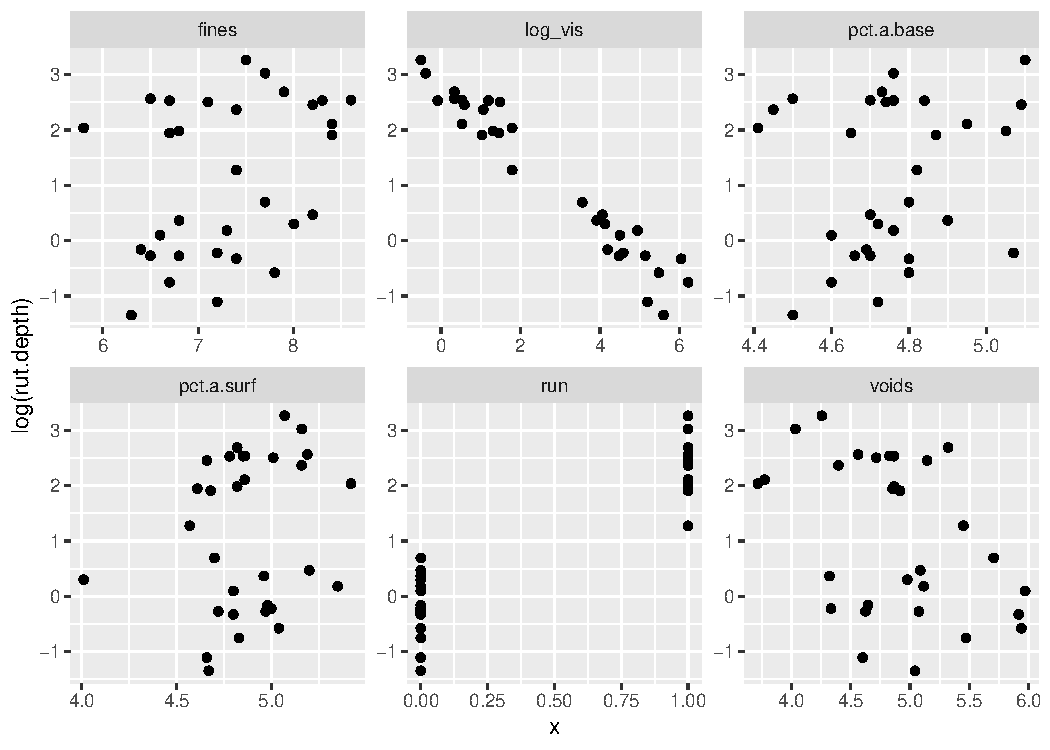
\includegraphics{asphalt_slides_files/figure-beamer/unnamed-chunk-20-1.pdf}
\end{frame}

\begin{frame}[fragile]{Modelling with transformed response}
\protect\hypertarget{modelling-with-transformed-response}{}
\begin{itemize}
\tightlist
\item
  These trends look pretty straight, especially with
  \texttt{log.viscosity}.
\item
  Values of \texttt{log.rut.depth} for each \texttt{run} have same
  spread.
\item
  Other trends weak, but are straight if they exist.
\item
  Start modelling from the beginning again.
\item
  Model \texttt{log.rut.depth} in terms of everything else, see what can
  be removed:
\end{itemize}

\begin{Shaded}
\begin{Highlighting}[]
\NormalTok{rut}\FloatTok{.2}\NormalTok{ \textless{}{-}}\StringTok{ }\KeywordTok{lm}\NormalTok{(}\KeywordTok{log}\NormalTok{(rut.depth) }\OperatorTok{\textasciitilde{}}\StringTok{ }\NormalTok{pct.a.surf }\OperatorTok{+}\StringTok{ }\NormalTok{pct.a.base }\OperatorTok{+}
\StringTok{  }\NormalTok{fines }\OperatorTok{+}\StringTok{ }\NormalTok{voids }\OperatorTok{+}\StringTok{ }\KeywordTok{log}\NormalTok{(viscosity) }\OperatorTok{+}\StringTok{ }\NormalTok{run, }\DataTypeTok{data =}\NormalTok{ asphalt)}
\end{Highlighting}
\end{Shaded}

\begin{itemize}
\tightlist
\item
  use \texttt{tidy} from \texttt{broom} to display just the
  coefficients.
\end{itemize}
\end{frame}

\begin{frame}[fragile]{Output}
\protect\hypertarget{output}{}
\begin{Shaded}
\begin{Highlighting}[]
\KeywordTok{tidy}\NormalTok{(rut}\FloatTok{.2}\NormalTok{)}
\end{Highlighting}
\end{Shaded}

\begin{longtable}[]{@{}lrrrr@{}}
\toprule
term & estimate & std.error & statistic & p.value\tabularnewline
\midrule
\endhead
(Intercept) & -1.5729892 & 2.4361740 & -0.6456802 &
0.5246124\tabularnewline
pct.a.surf & 0.5835756 & 0.2319811 & 2.5156167 &
0.0189818\tabularnewline
pct.a.base & -0.1033673 & 0.3689080 & -0.2801981 &
0.7817265\tabularnewline
fines & 0.0977520 & 0.0940682 & 1.0391609 & 0.3090864\tabularnewline
voids & 0.1988538 & 0.1230588 & 1.6159245 & 0.1191815\tabularnewline
log(viscosity) & -0.5576873 & 0.0854324 & -6.5278223 &
0.0000009\tabularnewline
run & 0.3400483 & 0.3388878 & 1.0034245 & 0.3256663\tabularnewline
\bottomrule
\end{longtable}
\end{frame}

\begin{frame}[fragile]{Taking out everything non-significant}
\protect\hypertarget{taking-out-everything-non-significant}{}
\begin{itemize}
\tightlist
\item
  Try: remove everything but pct.a.surf and log.viscosity:
\end{itemize}

\footnotesize

\begin{Shaded}
\begin{Highlighting}[]
\NormalTok{rut}\FloatTok{.3}\NormalTok{ \textless{}{-}}\StringTok{ }\KeywordTok{lm}\NormalTok{(}\KeywordTok{log}\NormalTok{(rut.depth) }\OperatorTok{\textasciitilde{}}\StringTok{ }\NormalTok{pct.a.surf }\OperatorTok{+}\StringTok{ }\KeywordTok{log}\NormalTok{(viscosity), }\DataTypeTok{data =}\NormalTok{ asphalt)}
\end{Highlighting}
\end{Shaded}

\normalsize

\footnotesize

\begin{itemize}
\tightlist
\item
  Check that removing all those variables wasn't too much:
\end{itemize}

\begin{Shaded}
\begin{Highlighting}[]
\KeywordTok{anova}\NormalTok{(rut}\FloatTok{.3}\NormalTok{, rut}\FloatTok{.2}\NormalTok{)}
\end{Highlighting}
\end{Shaded}

\begin{longtable}[]{@{}rrrrrr@{}}
\toprule
Res.Df & RSS & Df & Sum of Sq & F & Pr(\textgreater F)\tabularnewline
\midrule
\endhead
28 & 2.880919 & NA & NA & NA & NA\tabularnewline
24 & 2.288764 & 4 & 0.5921551 & 1.552336 & 0.2191461\tabularnewline
\bottomrule
\end{longtable}

\normalsize

\begin{itemize}
\tightlist
\item
  \(H_0\) : two models equally good; \(H_a\) : bigger model better.
\item
  Null not rejected here; small model as good as the big one, so prefer
  simpler smaller model \texttt{rut.3}.
\end{itemize}
\end{frame}

\begin{frame}[fragile]{Find the largest P-value by eye:}
\protect\hypertarget{find-the-largest-p-value-by-eye}{}
\begin{Shaded}
\begin{Highlighting}[]
\KeywordTok{tidy}\NormalTok{(rut}\FloatTok{.2}\NormalTok{)}
\end{Highlighting}
\end{Shaded}

\begin{longtable}[]{@{}lrrrr@{}}
\toprule
term & estimate & std.error & statistic & p.value\tabularnewline
\midrule
\endhead
(Intercept) & -1.5729892 & 2.4361740 & -0.6456802 &
0.5246124\tabularnewline
pct.a.surf & 0.5835756 & 0.2319811 & 2.5156167 &
0.0189818\tabularnewline
pct.a.base & -0.1033673 & 0.3689080 & -0.2801981 &
0.7817265\tabularnewline
fines & 0.0977520 & 0.0940682 & 1.0391609 & 0.3090864\tabularnewline
voids & 0.1988538 & 0.1230588 & 1.6159245 & 0.1191815\tabularnewline
log(viscosity) & -0.5576873 & 0.0854324 & -6.5278223 &
0.0000009\tabularnewline
run & 0.3400483 & 0.3388878 & 1.0034245 & 0.3256663\tabularnewline
\bottomrule
\end{longtable}

\begin{itemize}
\tightlist
\item
  Largest P-value is 0.78 for \texttt{pct.a.base}, not significant.
\item
  So remove this first, re-fit and re-assess.
\item
  Or, as over.
\end{itemize}
\end{frame}

\begin{frame}[fragile]{Get the computer to find the largest P-value for
you}
\protect\hypertarget{get-the-computer-to-find-the-largest-p-value-for-you}{}
\begin{itemize}
\tightlist
\item
  Output from \texttt{tidy} is itself a data frame, thus:
\end{itemize}

\begin{Shaded}
\begin{Highlighting}[]
\KeywordTok{tidy}\NormalTok{(rut}\FloatTok{.2}\NormalTok{) }\OperatorTok{\%\textgreater{}\%}\StringTok{ }\KeywordTok{arrange}\NormalTok{(p.value)}
\end{Highlighting}
\end{Shaded}

\begin{longtable}[]{@{}lrrrr@{}}
\toprule
term & estimate & std.error & statistic & p.value\tabularnewline
\midrule
\endhead
log(viscosity) & -0.5576873 & 0.0854324 & -6.5278223 &
0.0000009\tabularnewline
pct.a.surf & 0.5835756 & 0.2319811 & 2.5156167 &
0.0189818\tabularnewline
voids & 0.1988538 & 0.1230588 & 1.6159245 & 0.1191815\tabularnewline
fines & 0.0977520 & 0.0940682 & 1.0391609 & 0.3090864\tabularnewline
run & 0.3400483 & 0.3388878 & 1.0034245 & 0.3256663\tabularnewline
(Intercept) & -1.5729892 & 2.4361740 & -0.6456802 &
0.5246124\tabularnewline
pct.a.base & -0.1033673 & 0.3689080 & -0.2801981 &
0.7817265\tabularnewline
\bottomrule
\end{longtable}

\begin{itemize}
\tightlist
\item
  Largest P-value at the bottom.
\end{itemize}
\end{frame}

\begin{frame}[fragile]{Take out \texttt{pct.a.base}}
\protect\hypertarget{take-out-pct.a.base}{}
\begin{itemize}
\tightlist
\item
  Copy and paste the \texttt{lm} code and remove what you're removing:
\end{itemize}

\small

\begin{Shaded}
\begin{Highlighting}[]
\NormalTok{rut}\FloatTok{.4}\NormalTok{ \textless{}{-}}\StringTok{ }\KeywordTok{lm}\NormalTok{(}\KeywordTok{log}\NormalTok{(rut.depth) }\OperatorTok{\textasciitilde{}}\StringTok{ }\NormalTok{pct.a.surf }\OperatorTok{+}\StringTok{ }\NormalTok{fines }\OperatorTok{+}\StringTok{ }\NormalTok{voids }\OperatorTok{+}\StringTok{ }
\StringTok{              }\KeywordTok{log}\NormalTok{(viscosity) }\OperatorTok{+}\StringTok{ }\NormalTok{run, }\DataTypeTok{data =}\NormalTok{ asphalt)}
\KeywordTok{tidy}\NormalTok{(rut}\FloatTok{.4}\NormalTok{) }\OperatorTok{\%\textgreater{}\%}\StringTok{ }\KeywordTok{arrange}\NormalTok{(p.value)}
\end{Highlighting}
\end{Shaded}

\begin{longtable}[]{@{}lrrrr@{}}
\toprule
term & estimate & std.error & statistic & p.value\tabularnewline
\midrule
\endhead
log(viscosity) & -0.5524904 & 0.0818434 & -6.750578 &
0.0000004\tabularnewline
pct.a.surf & 0.5929947 & 0.2252626 & 2.632459 & 0.0143218\tabularnewline
voids & 0.2004674 & 0.1206373 & 1.661737 & 0.1090561\tabularnewline
(Intercept) & -2.0784987 & 1.6066507 & -1.293684 &
0.2075999\tabularnewline
run & 0.3597735 & 0.3253286 & 1.105877 & 0.2793085\tabularnewline
fines & 0.0889458 & 0.0870133 & 1.022209 & 0.3164725\tabularnewline
\bottomrule
\end{longtable}

\normalsize

\begin{itemize}
\tightlist
\item
  \texttt{fines} is next to go, P-value 0.32.
\end{itemize}
\end{frame}

\begin{frame}[fragile]{``Update''}
\protect\hypertarget{update}{}
Another way to do the same thing:

\begin{Shaded}
\begin{Highlighting}[]
\NormalTok{rut}\FloatTok{.4}\NormalTok{ \textless{}{-}}\StringTok{ }\KeywordTok{update}\NormalTok{(rut}\FloatTok{.2}\NormalTok{, . }\OperatorTok{\textasciitilde{}}\StringTok{ }\NormalTok{. }\OperatorTok{{-}}\StringTok{ }\NormalTok{pct.a.base)}
\KeywordTok{tidy}\NormalTok{(rut}\FloatTok{.4}\NormalTok{) }\OperatorTok{\%\textgreater{}\%}\StringTok{ }\KeywordTok{arrange}\NormalTok{(p.value)}
\end{Highlighting}
\end{Shaded}

\begin{longtable}[]{@{}lrrrr@{}}
\toprule
term & estimate & std.error & statistic & p.value\tabularnewline
\midrule
\endhead
log(viscosity) & -0.5524904 & 0.0818434 & -6.750578 &
0.0000004\tabularnewline
pct.a.surf & 0.5929947 & 0.2252626 & 2.632459 & 0.0143218\tabularnewline
voids & 0.2004674 & 0.1206373 & 1.661737 & 0.1090561\tabularnewline
(Intercept) & -2.0784987 & 1.6066507 & -1.293684 &
0.2075999\tabularnewline
run & 0.3597735 & 0.3253286 & 1.105877 & 0.2793085\tabularnewline
fines & 0.0889458 & 0.0870133 & 1.022209 & 0.3164725\tabularnewline
\bottomrule
\end{longtable}

\begin{itemize}
\tightlist
\item
  Again, fines is the one to go. (Output identical as it should be.)
\end{itemize}
\end{frame}

\begin{frame}[fragile]{Take out fines:}
\protect\hypertarget{take-out-fines}{}
\begin{Shaded}
\begin{Highlighting}[]
\NormalTok{rut}\FloatTok{.5}\NormalTok{ \textless{}{-}}\StringTok{ }\KeywordTok{update}\NormalTok{(rut}\FloatTok{.4}\NormalTok{, . }\OperatorTok{\textasciitilde{}}\StringTok{ }\NormalTok{. }\OperatorTok{{-}}\StringTok{ }\NormalTok{fines)}
\KeywordTok{tidy}\NormalTok{(rut}\FloatTok{.5}\NormalTok{) }\OperatorTok{\%\textgreater{}\%}\StringTok{ }\KeywordTok{arrange}\NormalTok{(p.value)}
\end{Highlighting}
\end{Shaded}

\begin{longtable}[]{@{}lrrrr@{}}
\toprule
term & estimate & std.error & statistic & p.value\tabularnewline
\midrule
\endhead
log(viscosity) & -0.5803887 & 0.0772254 & -7.5155118 &
0.0000001\tabularnewline
pct.a.surf & 0.5483723 & 0.2211833 & 2.4792668 &
0.0199713\tabularnewline
voids & 0.2318797 & 0.1167584 & 1.9859780 & 0.0576740\tabularnewline
run & 0.2946793 & 0.3193108 & 0.9228604 & 0.3645654\tabularnewline
(Intercept) & -1.2553309 & 1.3914683 & -0.9021628 &
0.3752525\tabularnewline
\bottomrule
\end{longtable}

Can't take out intercept, so \texttt{run}, with P-value 0.36, goes next.
\end{frame}

\begin{frame}[fragile]{Take out run:}
\protect\hypertarget{take-out-run}{}
\begin{Shaded}
\begin{Highlighting}[]
\NormalTok{rut}\FloatTok{.6}\NormalTok{ \textless{}{-}}\StringTok{ }\KeywordTok{update}\NormalTok{(rut}\FloatTok{.5}\NormalTok{, . }\OperatorTok{\textasciitilde{}}\StringTok{ }\NormalTok{. }\OperatorTok{{-}}\StringTok{ }\NormalTok{run)}
\KeywordTok{tidy}\NormalTok{(rut}\FloatTok{.6}\NormalTok{) }\OperatorTok{\%\textgreater{}\%}\StringTok{ }\KeywordTok{arrange}\NormalTok{(p.value)}
\end{Highlighting}
\end{Shaded}

\begin{longtable}[]{@{}lrrrr@{}}
\toprule
term & estimate & std.error & statistic & p.value\tabularnewline
\midrule
\endhead
log(viscosity) & -0.6464911 & 0.0287864 & -22.4581853 &
0.0000000\tabularnewline
pct.a.surf & 0.5554686 & 0.2204415 & 2.5198000 &
0.0179633\tabularnewline
voids & 0.2447934 & 0.1155981 & 2.1176259 & 0.0435604\tabularnewline
(Intercept) & -1.0207945 & 1.3643000 & -0.7482185 &
0.4607966\tabularnewline
\bottomrule
\end{longtable}

Again, can't take out intercept, so largest P-value is for
\texttt{voids}, 0.044. But this is significant, so we shouldn't remove
\texttt{voids}.
\end{frame}

\begin{frame}[fragile]{Comments}
\protect\hypertarget{comments-2}{}
\begin{itemize}
\tightlist
\item
  Here we stop: \texttt{pct.a.surf}, \texttt{voids} and
  \texttt{log.viscosity} would all make fit significantly worse if
  removed. So they stay.
\item
  Different final result from taking things out one at a time (top),
  than by taking out 4 at once (bottom):
\end{itemize}

\begin{Shaded}
\begin{Highlighting}[]
\KeywordTok{coef}\NormalTok{(rut}\FloatTok{.6}\NormalTok{)}
\end{Highlighting}
\end{Shaded}

\begin{verbatim}
##    (Intercept)     pct.a.surf          voids 
##     -1.0207945      0.5554686      0.2447934 
## log(viscosity) 
##     -0.6464911
\end{verbatim}

\begin{Shaded}
\begin{Highlighting}[]
\KeywordTok{coef}\NormalTok{(rut}\FloatTok{.3}\NormalTok{)}
\end{Highlighting}
\end{Shaded}

\begin{verbatim}
##    (Intercept)     pct.a.surf log(viscosity) 
##      0.9001389      0.3911481     -0.6185628
\end{verbatim}

\begin{itemize}
\tightlist
\item
  Point: Can make difference which way we go.
\end{itemize}
\end{frame}

\begin{frame}[fragile]{Comments on variable selection}
\protect\hypertarget{comments-on-variable-selection}{}
\begin{itemize}
\tightlist
\item
  Best way to decide which \(x\)'s belong: expert knowledge: which of
  them should be important.
\item
  Best automatic method: what we did, ``backward selection''.
\item
  Do not learn about ``stepwise regression''!
  \href{https://towardsdatascience.com/stopping-stepwise-why-stepwise-selection-is-bad-and-what-you-should-use-instead-90818b3f52df}{\textbf{eg.
  here}}
\item
  R has function \texttt{step} that does backward selection, like this:
\end{itemize}

\begin{Shaded}
\begin{Highlighting}[]
\KeywordTok{step}\NormalTok{(rut}\FloatTok{.2}\NormalTok{, }\DataTypeTok{direction =} \StringTok{"backward"}\NormalTok{, }\DataTypeTok{test =} \StringTok{"F"}\NormalTok{)}
\end{Highlighting}
\end{Shaded}

Gets same answer as we did (by removing least significant x).

\begin{itemize}
\tightlist
\item
  Removing non-significant \(x\)'s may remove interesting ones whose
  P-values happened not to reach 0.05. Consider using less stringent
  cutoff like 0.20 or even bigger.
\item
  Can also fit all possible regressions, as over (may need to do
  \texttt{install.packages("leaps")} first).
\end{itemize}
\end{frame}

\begin{frame}[fragile]{All possible regressions (output over)}
\protect\hypertarget{all-possible-regressions-output-over}{}
Uses package \texttt{leaps}:

\begin{Shaded}
\begin{Highlighting}[]
\NormalTok{leaps \textless{}{-}}\StringTok{ }\KeywordTok{regsubsets}\NormalTok{(}\KeywordTok{log}\NormalTok{(rut.depth) }\OperatorTok{\textasciitilde{}}\StringTok{ }\NormalTok{pct.a.surf }\OperatorTok{+}\StringTok{ }
\StringTok{                      }\NormalTok{pct.a.base }\OperatorTok{+}\StringTok{ }\NormalTok{fines }\OperatorTok{+}\StringTok{ }\NormalTok{voids }\OperatorTok{+}\StringTok{ }
\StringTok{                      }\KeywordTok{log}\NormalTok{(viscosity) }\OperatorTok{+}\StringTok{ }\NormalTok{run, }
                    \DataTypeTok{data =}\NormalTok{ asphalt, }\DataTypeTok{nbest =} \DecValTok{2}\NormalTok{)}
\NormalTok{s \textless{}{-}}\StringTok{ }\KeywordTok{summary}\NormalTok{(leaps)}
\KeywordTok{with}\NormalTok{(s, }\KeywordTok{data.frame}\NormalTok{(rsq, outmat)) {-}\textgreater{}}\StringTok{ }\NormalTok{d}
\end{Highlighting}
\end{Shaded}
\end{frame}

\begin{frame}[fragile]{The output}
\protect\hypertarget{the-output}{}
\scriptsize

\begin{Shaded}
\begin{Highlighting}[]
\NormalTok{d }\OperatorTok{\%\textgreater{}\%}\StringTok{ }\KeywordTok{rownames\_to\_column}\NormalTok{(}\StringTok{"model"}\NormalTok{) }\OperatorTok{\%\textgreater{}\%}\StringTok{ }\KeywordTok{arrange}\NormalTok{(}\KeywordTok{desc}\NormalTok{(rsq))}
\end{Highlighting}
\end{Shaded}

\begin{longtable}[]{@{}lrllllll@{}}
\toprule
model & rsq & pct.a.surf & pct.a.base & fines & voids & log.viscosity. &
run\tabularnewline
\midrule
\endhead
6 ( 1 ) & 0.9609642 & * & * & * & * & * & *\tabularnewline
5 ( 1 ) & 0.9608365 & * & & * & * & * & *\tabularnewline
5 ( 2 ) & 0.9593265 & * & * & * & * & * &\tabularnewline
4 ( 1 ) & 0.9591996 & * & & & * & * & *\tabularnewline
4 ( 2 ) & 0.9589206 & * & & * & * & * &\tabularnewline
3 ( 1 ) & 0.9578631 & * & & & * & * &\tabularnewline
3 ( 2 ) & 0.9534561 & * & & * & & * &\tabularnewline
2 ( 1 ) & 0.9508647 & * & & & & * &\tabularnewline
2 ( 2 ) & 0.9479541 & & & & * & * &\tabularnewline
1 ( 1 ) & 0.9452562 & & & & & * &\tabularnewline
1 ( 2 ) & 0.8624107 & & & & & & *\tabularnewline
\bottomrule
\end{longtable}

\normalsize
\end{frame}

\begin{frame}[fragile]{Comments}
\protect\hypertarget{comments-3}{}
\begin{itemize}
\tightlist
\item
  Problem: even adding a worthless x increases R-squared. So try for
  line where R-squared stops increasing ``too much'', eg. top line (just
  log.viscosity), first 3-variable line (backwards-elimination model).
  Hard to judge.
\item
  One solution (STAC67): adjusted R-squared, where adding worthless
  variable makes it go down.
\item
  \texttt{data.frame} rather than \texttt{tibble} because there are
  several columns in \texttt{outmat}.
\end{itemize}
\end{frame}

\begin{frame}[fragile]{All possible regressions, adjusted R-squared}
\protect\hypertarget{all-possible-regressions-adjusted-r-squared}{}
\scriptsize

\begin{Shaded}
\begin{Highlighting}[]
\KeywordTok{with}\NormalTok{(s, }\KeywordTok{data.frame}\NormalTok{(adjr2, outmat)) }\OperatorTok{\%\textgreater{}\%}\StringTok{ }
\StringTok{  }\KeywordTok{rownames\_to\_column}\NormalTok{(}\StringTok{"model"}\NormalTok{) }\OperatorTok{\%\textgreater{}\%}\StringTok{ }
\StringTok{  }\KeywordTok{arrange}\NormalTok{(}\KeywordTok{desc}\NormalTok{(adjr2))}
\end{Highlighting}
\end{Shaded}

\begin{longtable}[]{@{}lrllllll@{}}
\toprule
model & adjr2 & pct.a.surf & pct.a.base & fines & voids & log.viscosity.
& run\tabularnewline
\midrule
\endhead
3 ( 1 ) & 0.9531812 & * & & & * & * &\tabularnewline
5 ( 1 ) & 0.9530038 & * & & * & * & * & *\tabularnewline
4 ( 1 ) & 0.9529226 & * & & & * & * & *\tabularnewline
4 ( 2 ) & 0.9526007 & * & & * & * & * &\tabularnewline
6 ( 1 ) & 0.9512052 & * & * & * & * & * & *\tabularnewline
5 ( 2 ) & 0.9511918 & * & * & * & * & * &\tabularnewline
3 ( 2 ) & 0.9482845 & * & & * & & * &\tabularnewline
2 ( 1 ) & 0.9473550 & * & & & & * &\tabularnewline
2 ( 2 ) & 0.9442365 & & & & * & * &\tabularnewline
1 ( 1 ) & 0.9433685 & & & & & * &\tabularnewline
1 ( 2 ) & 0.8576662 & & & & & & *\tabularnewline
\bottomrule
\end{longtable}

\normalsize
\end{frame}

\begin{frame}[fragile]{Revisiting the best model}
\protect\hypertarget{revisiting-the-best-model}{}
\begin{itemize}
\tightlist
\item
  Best model was our rut.6:
\end{itemize}

\begin{Shaded}
\begin{Highlighting}[]
\KeywordTok{tidy}\NormalTok{(rut}\FloatTok{.6}\NormalTok{)}
\end{Highlighting}
\end{Shaded}

\begin{longtable}[]{@{}lrrrr@{}}
\toprule
term & estimate & std.error & statistic & p.value\tabularnewline
\midrule
\endhead
(Intercept) & -1.0207945 & 1.3643000 & -0.7482185 &
0.4607966\tabularnewline
pct.a.surf & 0.5554686 & 0.2204415 & 2.5198000 &
0.0179633\tabularnewline
voids & 0.2447934 & 0.1155981 & 2.1176259 & 0.0435604\tabularnewline
log(viscosity) & -0.6464911 & 0.0287864 & -22.4581853 &
0.0000000\tabularnewline
\bottomrule
\end{longtable}
\end{frame}

\begin{frame}[fragile]{Revisiting (2)}
\protect\hypertarget{revisiting-2}{}
\begin{itemize}
\tightlist
\item
  Regression slopes say that rut depth increases as log-viscosity
  decreases, \texttt{pct.a.surf} increases and \texttt{voids} increases.
  This more or less checks out with out scatterplots against
  \texttt{log.viscosity}.
\item
  We should check residual plots again, though previous scatterplots say
  it's unlikely that there will be a problem:
\end{itemize}

\begin{Shaded}
\begin{Highlighting}[]
\NormalTok{g \textless{}{-}}\StringTok{ }\KeywordTok{ggplot}\NormalTok{(rut}\FloatTok{.6}\NormalTok{, }\KeywordTok{aes}\NormalTok{(}\DataTypeTok{y =}\NormalTok{ .resid, }\DataTypeTok{x =}\NormalTok{ .fitted)) }\OperatorTok{+}\StringTok{ }
\KeywordTok{geom\_point}\NormalTok{()}
\end{Highlighting}
\end{Shaded}
\end{frame}

\begin{frame}[fragile]{Residuals against fitted values}
\protect\hypertarget{residuals-against-fitted-values}{}
\begin{Shaded}
\begin{Highlighting}[]
\NormalTok{g}
\end{Highlighting}
\end{Shaded}

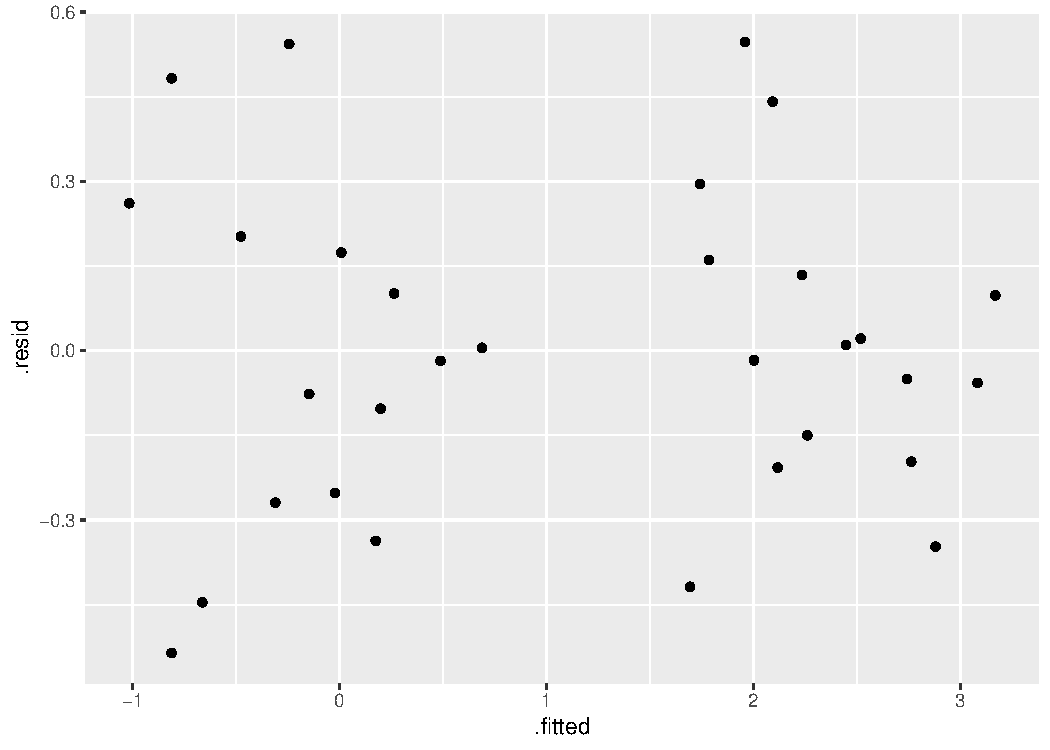
\includegraphics{asphalt_slides_files/figure-beamer/unnamed-chunk-42-1.pdf}
\end{frame}

\begin{frame}[fragile]{Plotting residuals against x's}
\protect\hypertarget{plotting-residuals-against-xs}{}
\begin{itemize}
\tightlist
\item
  Do our trick again to put them all on one plot:
\end{itemize}

\begin{Shaded}
\begin{Highlighting}[]
\KeywordTok{augment}\NormalTok{(rut}\FloatTok{.6}\NormalTok{, asphalt) }\OperatorTok{\%\textgreater{}\%}
\StringTok{  }\KeywordTok{mutate}\NormalTok{(}\DataTypeTok{log\_vis=}\KeywordTok{log}\NormalTok{(viscosity)) }\OperatorTok{\%\textgreater{}\%}\StringTok{ }
\StringTok{  }\KeywordTok{pivot\_longer}\NormalTok{(}
    \KeywordTok{c}\NormalTok{(pct.a.surf}\OperatorTok{:}\NormalTok{voids, run, log\_vis),}
    \DataTypeTok{names\_to=}\StringTok{"xname"}\NormalTok{, }\DataTypeTok{values\_to=}\StringTok{"x"}\NormalTok{,}
\NormalTok{  ) }\OperatorTok{\%\textgreater{}\%}
\StringTok{  }\KeywordTok{ggplot}\NormalTok{(}\KeywordTok{aes}\NormalTok{(}\DataTypeTok{y =}\NormalTok{ .resid, }\DataTypeTok{x =}\NormalTok{ x)) }\OperatorTok{+}\StringTok{ }\KeywordTok{geom\_point}\NormalTok{() }\OperatorTok{+}
\StringTok{  }\KeywordTok{facet\_wrap}\NormalTok{(}\OperatorTok{\textasciitilde{}}\NormalTok{xname, }\DataTypeTok{scales =} \StringTok{"free"}\NormalTok{) {-}\textgreater{}}\StringTok{ }\NormalTok{g2}
\end{Highlighting}
\end{Shaded}
\end{frame}

\begin{frame}[fragile]{Residuals against the x's}
\protect\hypertarget{residuals-against-the-xs}{}
\begin{Shaded}
\begin{Highlighting}[]
\NormalTok{g2}
\end{Highlighting}
\end{Shaded}

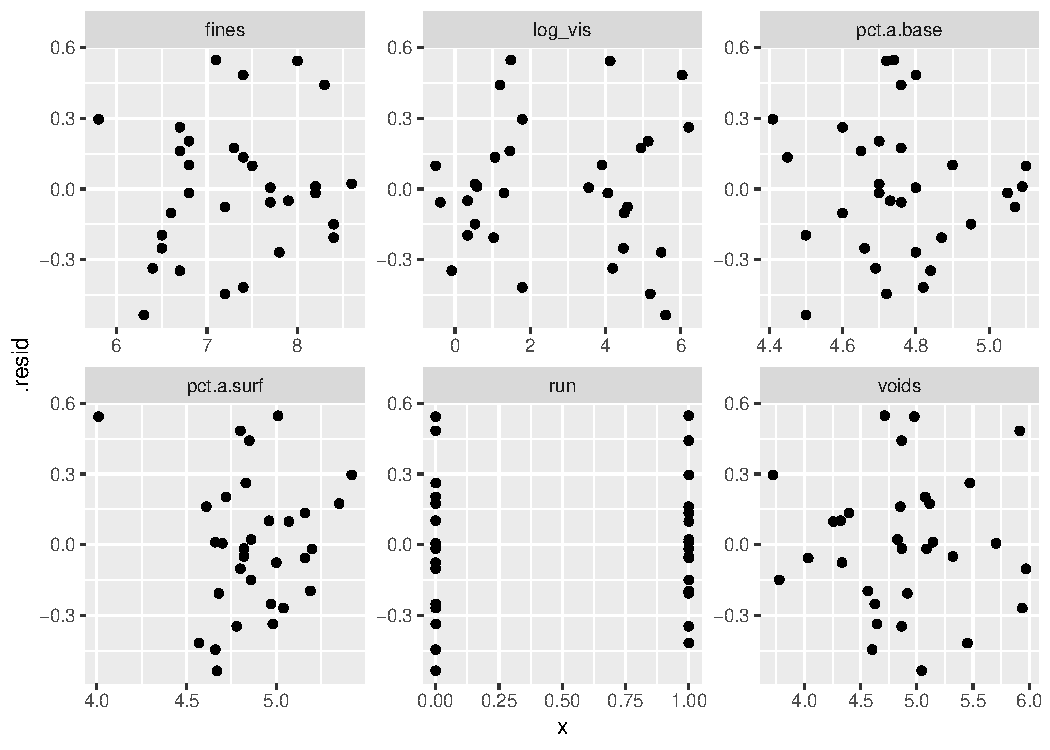
\includegraphics{asphalt_slides_files/figure-beamer/unnamed-chunk-44-1.pdf}
\end{frame}

\begin{frame}{Comments}
\protect\hypertarget{comments-4}{}
\begin{itemize}
\tightlist
\item
  None of the plots show any sort of pattern. The points all look random
  on each plot.
\item
  On the plot of fitted values (and on the one of log.viscosity), the
  points seem to form a ``left half'' and a ``right half'' with a gap in
  the middle. This is not a concern.
\item
  One of the pct.a.surf values is low outlier (4), shows up top left of
  that plot.
\item
  Only two possible values of run; the points in each group look
  randomly scattered around 0, with equal spreads.
\item
  Residuals seem to go above zero further than below, suggesting a mild
  non-normality, but not enough to be a problem.
\end{itemize}
\end{frame}

\begin{frame}{Variable-selection strategies}
\protect\hypertarget{variable-selection-strategies}{}
\begin{itemize}
\tightlist
\item
  Expert knowledge.
\item
  Backward elimination.
\item
  All possible regressions.
\item
  Taking a variety of models to experts and asking their opinion.
\item
  Use a looser cutoff to eliminate variables in backward elimination
  (eg. only if P-value greater than 0.20).
\item
  If goal is prediction, eliminating worthless variables less important.
\item
  If goal is understanding, want to eliminate worthless variables where
  possible.
\item
  Results of variable selection not always reproducible, so caution
  advised.
\end{itemize}
\end{frame}
